% siminos/presentations/MATT18/MATT18.tex pdflatex MATT18; biber MATT18
% $Author: predrag $ $Date: 2018-11-30 12:00:26 -0500 (Fri, 30 Nov 2018) $

%% started with siminos/gudorf/thesis/proposal/tex/ppt.tex
%% logical setup, no need to edit %%%%%%%%%%
\newif\ifpaper \newif\ifPDF               %%
\newif\ifOUP \newif\ifboyscout            %%
\newif\ifdasbuch \newif\ifarticle         %%
\newif\ifsolutions

\newif\ifbackground % whether use background image
\backgroundfalse
\newif\iflogo % whether use logo
\logotrue
\newif\ifnotes % whether show notes.
\notesfalse
\newif\ifhandout % handout mode
\handoutfalse
%%%%%%%%%%%%%%%%%%%%%%%%%%%%%%%%%%%%%%%%%%%%%%%%%%%%%%%%%%%%%%%%%%%%%%

\ifhandout
\documentclass[mathserif, handout]{beamer}
\else
\documentclass[mathserif]{beamer}
\fi

\usepackage{graphicx}
\usepackage{algpseudocode}
\usepackage{algorithm}
\usepackage{tikz}
\usetikzlibrary{calc}
\usetikzlibrary{decorations.pathreplacing}
\usepackage{tipa}
\usepackage[font=small,labelfont=bf]{caption}
\usepackage{subcaption}
\usepackage{amsthm}

\usepackage[
    backend=biber,  %bibtex,
    sorting=nyt,
    %refsection=chapter,
    %citereset=chapter,
    style=numeric, %alphabetic, % %style=authoryear,
    natbib=true,
    style=phys, % aps
    biblabel= brackets, % superscript, %
    articletitle=false, % true,  % false, % aps
    %chaptertitle=true,  % aip;  % false, % aps
    pageranges = true , % aip: the full range
             % = false, % aps: only the first page being printed
    sortlocale=en_US,
    firstinits=true,
    url=false, %true,  %
    doi=false, %true,
    eprint=false
]{biblatex}
\addbibresource{../../bibtex/siminos.bib}

%%%%%%%%%%%%%%%%%%%%%%%%%%%%%%%%%%%%%%%%%%%%%%%%%%%%%%%%%%%%%%%%%%%%%%
% deal with the conflicts between def.tex and beamer
\newcounter{chapter}
\let\block\undefined
\let\Loop\undefined
\let\definition\undefined
\let\theorem\undefined
\let\lemma\undefined

\input{../../inputs/def}            %% do not edit; update from
\input{../../inputs/editsDasbuch}   %% editing comments, DasBuch style
%\input ../../inputs/defsSpatiotemp
% siminos/gudorf/thesis/defsThesis.tex
% $Author: predrag $ $Date: 2018-11-02 16:08:17 -0400 (Fri, 02 Nov 2018) $

\ifboyscout %%%%%%%% DISPLAY COMMENTS IN THE TEXT %%%%%%%%%%%%%%%%%%%%
            %%%%%%%% turn on labeling of equations on margins %%%%%%%%
    % also search the text for lines starting with %%  to
    % locate various internal comments, recent edits etc.
    \typeout{============ COMMENTED =====}
 \renewcommand{\PC}[2]{$\footnotemark\footnotetext{Predrag #1: #2}$} %date, comment
 \newcommand{\AC}[2]{$\footnotemark\footnotetext{Andy #1: #2}$} %date, comment
 \newcommand{\BG}[2]{$\footnotemark\footnotetext{Boris #1: #2}$} %date, comment
 \renewcommand{\AKS}[2]{$\footnotemark\footnotetext{Adrien #1: #2}$} %date, comment
 \renewcommand{\RJ}[2]{$\footnotemark\footnotetext{Rana #1: #2}$} %date, comment
 \renewcommand{\HL}[2]{$\footnotemark\footnotetext{Han #1: #2}$} %date, comment
 \newcommand{\MNG}[2]{$\footnotemark\footnotetext{Matt #1: #2}$} %date, comment
\else % drop comments
      % do not turn on labeling of equations on margins
  \typeout{============ UNCOMMENTED =====}
 \renewcommand{\PC}[2]{}
 \newcommand{\AC}[2]{}
 \newcommand{\BG}[2]{}
 \renewcommand{\AKS}[2]{}
 \renewcommand{\RJ}[2]{}
 \renewcommand{\HL}[2]{}
 \newcommand{\MNG}[2]{}
\fi  %%%%%%%%%%%% END OF ON/OFF COMMENTS SWITCH %%%%%%%%%%%%%%%%%%%%

%\newcommand{\YTlink}[1]{\marginpar{   %% links to YouTube videos
%    \HREF{http://#1}{\includegraphics[width=16pt]{start-32}}}
%                       }
\newcommand{\YTlink}[1]{    %% in text, links to YouTube videos
    \raisebox{-0.4ex}[0pt][0pt]{\!\!\!
    \HREF{http://#1}{\includegraphics[height=1em]{start-32}}
    \!\!\!            }  }
% in-text pointer to a video   2014-01-18
\newcommand{\videoLink}[1]{    %% in text, links to YouTube videos
    \raisebox{-0.4ex}[0pt][0pt]{$\!\!\!$
    \HREF{http://#1}{\includegraphics[height=1em]{YouTubeIcon}}
                    % or maybe streamThisRed}}
                    % do not have compact eps for {start-32}
    $\!$             }}
% in-text pointer to a video   2014-01-18
\newcommand{\toVideo}[1]
{\marginpar[\videoLink{#1}]{\videoLink{#1} \hfill}}

% \renewcommand{\toChap}[1]{}
\renewcommand{\cl}[1]{{\ensuremath{|#1|}}}  % the length of a periodic orbit, Ronnie
%\newcommand{\XD}{Xiong Ding}

\ifpaper % prepare for B&W paper printing:
       \renewcommand{\arXiv}[1]{ {arXiv:#1}}
\else % prepare hyperlinked pdf
       \renewcommand{\arXiv}[1]{
              {\href{http://arXiv.org/abs/#1}{arXiv:#1}}}
\fi

    \ifboyscout
\newcommand{\toCB}{\marginpar{\footnotesize 2CB}}  % to compare with ChaosBook
\newcommand{\inCB}{\marginpar{\footnotesize now in CB}} % entered in ChaosBook
\newcommand{\CBlibrary}[1]
{\href{http://ChaosBook.org/library/#1.pdf} { (click here)}}
    \else
\newcommand{\toCB}{}
\newcommand{\inCB}{}
\newcommand{\CBlibrary}[1]{}
    \fi %end of internal draft switch

\newcommand{\conf}{\ensuremath{x}}      % Configuration space coordinate
\newcommand{\Fu}{\tilde{u}}
\newcommand{\abs}[1]{\lvert#1\rvert}    % Absolute value
\newcommand{\twot}{invariant 2-torus} % Predrag, to distinguish from a PO
\newcommand{\twots}{invariant 2-tori}
\newcommand{\twoT}{Invariant 2-torus}
\newcommand{\twoTs}{Invariant 2-tori}
\newcommand{\brick}{block}
\newcommand{\Brick}{Block}
\renewcommand{\action}{W}                 % PC 07jan2018
% \newcommand{\action}{S}               % Boris
%\newcommand{\genF}{F}                  % Li and Tomsovic generating function
\newcommand{\genF}{L}                   % McKay generating function

%%%%%% Boris definitions
\newcommand{\Aa}{\ensuremath{\bar{\A}}}
\newcommand{\A}{\ensuremath{\mathcal{A}}}       % alphabet
\newcommand{\Ai}{\ensuremath{\mathcal{A}_0}}    % alphabet inner
\newcommand{\Ae}{\ensuremath{\mathcal{A}_1}}    % alphabet outer
\newcommand{\R}{\ensuremath{\mathcal{R}}}
%\newcommand{\m}{\ensuremath{\mathsf{m}}}     % Boris
\newcommand{\m}{\ensuremath{m}}     % Predrag experimental 2016-11-08
\newcommand{\Mm}{\ensuremath{\mathsf{M}}}
\newcommand{\Xx}{\ensuremath{\mathsf{X}}}
\newcommand{\Zz}{\ensuremath{\mathbb{Z}^2}}
\newcommand{\ZLT}{\mathbb{Z}^2_{\scriptscriptstyle\mathrm{LT}}}
%\newcommand{\q}{\ensuremath{\mathsf{m}}}     % Boris
\newcommand{\q}{\ensuremath{q}}     % Predrag experimental 2016-11-08
\newcommand{\D}{\mathcal{D}}
\newcommand{\gd}{\mathsf{g}}
\newcommand{\gp}{\mathsf{g}^0}

%%%%%%%%%%%% MACROS, Xiong Ding specific %%%%%%%%%%
\DeclareMathOperator{\im}{Im}
\DeclareMathOperator{\re}{Re}
\DeclareMathOperator{\diag}{Diag}
\DeclareMathOperator{\dist}{dist}
\DeclareMathOperator{\const}{const}
% ==============================
\newcommand{\spt}{spatiotemporal}
\newcommand{\Spt}{Spatiotemporal}
\newcommand{\xDFt}{Discrete Fourier transform}
\newcommand{\xdFt}{discrete Fourier transform}

\newcommand{\cGL}{complex Ginzburg-Landau}
\newcommand{\cGLe}{complex Ginzburg-Landau equation}


%%%%%%%%%%%% MACROS, Siminos specific %%%%%%%%%%
\newcommand{\edit}[1]{{\color{blue} #1}} % for referees
%\newcommand{\edit}[1]{#1}               % for the journal
\newcommand{\vf}{v}	%%% keep notation for vector field flexible.
                    % For the time being follow Das Buch.
\newcommand{\conj}[1]{\ensuremath{\bar{#1}}}
\newcommand{\Manif}{\ensuremath{\mathcal{M}}}
\newcommand{\Order}[1]{\mathrm{O}(#1)}
\newcommand{\steady}{\textdollar~}

%%%%%%%% Symmetries, Siminos specific %%%%%%%%%%
%\renewcommand{\shift}{\ensuremath{\ell}}
%\newcommand{\Shift}{\ensuremath{\tau}}
\newcommand{\Idg}{\ensuremath{\mathbf{1}}}
\newcommand{\En}[1]{\ensuremath{\mathrm{E}(#1)}}
\newcommand{\Rotn}[1]{\ensuremath{R_{#1}}}
\newcommand{\Drot}{\ensuremath{\zeta}}
\newcommand{\globstab}[1]{\ensuremath{\Sigma_{#1}}} % Change to be the same as stab. Was \Sigma^\ast_{#1}
\newcommand{\Str}[1]{\ensuremath{\mathcal{S}_{#1}}} % Stratum
\newcommand{\Nlz}[1]{\ensuremath{N(#1)}}
\newcommand{\doubleperiod}[1]{{\ensuremath{\mathcal{T}_{#1}}}}

%%%%%%%%%%%% Theorems, Siminos specific %%%%%%%%%%
%%%%%%%%%%%%%% Solution labels %%%%%%%%%%%%%%%%%%%%


% Redefine using mathrm, it is a label not a math symbol
\renewcommand{\EQV}[1]{\ensuremath{\mathrm{E}_{#1}}}
% E_0: u = 0 - trivial equilibrium
% E_1,E_2,E_3, for 1,2,3-wave equilibria
\renewcommand{\REQV}[2]{\ensuremath{\mathrm{TW}_{#1#2}}} % #1 is + or -
% TW_1^{+,-} for 1-wave traveling waves (positive and negative velocity).
\renewcommand{\PO}[1]{\ensuremath{\mathrm{PO}_{#1}}}
% PO_{period to 2-4 significant digits} - periodic orbits
\renewcommand{\RPO}[1]{\ensuremath{\mathrm{RPO}_{#1}}}
% RPO_{period to 2-4 significant digits} - relative PO.  We use ^{+,-}
% to distinguish between members of a reflection-symmetric pair.
% Gibson likes:
\renewcommand{\tEQ}{\ensuremath{\mathrm{EQ}}}

\newcommand{\tLB}{\ensuremath{{\text{EQ}_1}}}
\newcommand{\tUB}{\ensuremath{{\text{EQ}_2}}}

%%%%%%%%%%%%%% Operators %%%%%%%%%%%%%%%%%%%%%%%
\newcommand{\PperpOp}{\mathbf{P}^{\perp}}
%\newcommand{\Pperp}{P^{\perp}}
%

%%%%%%%%%%% Equations, Siminos specific %%%%%%%%%%
\newcommand{\cont}{\,, \\ }

%%%%%%%%%%%%%%%%%%%%%%%%%%%%%%%%%%%%%%%%%%%%%%%%%%%%%%%%%%%
% JFG favorite macros
\newcommand{\bu}{\ensuremath{{\bf u}}}
\newcommand{\bx}{{\bf x}}
\newcommand{\trHalf}[1]{\tau_{#1}}    % 1/2 cell translation
\newcommand{\GPCF}{\ensuremath{\Gamma}} % Hoyle notation, equivariant symmetry group

%%%%%%%%%%%%%%%%%%%%%%%%%%%%%%%%%%%%%%%%%%%%%%%%%%%%%%%%%%%
% GUDORF specific macros.
\newcommand{\F}{\ensuremath{\mathcal{F}}}
\newcommand{\Fi}{\ensuremath{\mathcal{F}^{-1}}}
\newcommand{\Dxx}{\ensuremath{\mathcal{D}_{\conf \conf}}}
\newcommand{\Dfourx}{\ensuremath{\mathcal{D}_{\conf \conf \conf \conf}}}
\newcommand{\Sop}{\ensuremath{\mathcal{S}}}
\newcommand{\Dt}{\ensuremath{\mathcal{D}_{\zeit}}}
\newcommand{\Dx}{\ensuremath{\mathcal{D}_{\conf}}}
\newcommand{\ufield}{\ensuremath{u(\conf,\zeit)}}
\newcommand{\dufield}{\ensuremath{u(\conf_{m},\zeit_{n})}}
\newcommand{\sFb}{spatiotemporal Fourier basis}
\newcommand{\rv}{real valued}
\newcommand{\Fuvec}{\ensuremath{\mathbf{\tilde{u}}}}
\newcommand{\umn}{\ensuremath{\tilde{u}_{\sss{m,n}}}}
\newcommand{\nm}[1]{\tilde{{#1}}_{\sss{n,m}}}
\newcommand{\qm}{\ensuremath{q_{\sss m}}}
\newcommand{\wavevec}{\ensuremath{\frac{2\pi m}{L}}}
\newcommand{\wn}{\ensuremath{\omega_{\sss n}}}
\newcommand{\freqvec}{\ensuremath{\frac{2\pi n}{T}}}

%%%%%%%%%%%%%%%%%%%%%%%%%%%%%%%%%%%%%%%%%%%%%%%%%%%%%%%%%%%
% Lopez favorite macros, REMOVE MOST EVENTUALLY
\newcommand{\sss}{\scriptscriptstyle}	
\newcommand{\e}{\mathrm{e}}
\newcommand{\mmbf}[1]{\mbox{\boldmath ${#1}$}}
\newcommand{\Arot}{\theta}
\newcommand{\spacetrans}{\sigma}
\newcommand{\timetrans}{\tau}
\newcommand{\lsym}{l}
\newcommand{\ce}{c_{\sss{1}}}
\newcommand{\co}{c_{\sss{2}}}
\newcommand{\Lx}{L_{\sss x}}
\newcommand{\omegan}{\omega_{\sss n}}
\newcommand{\km}{k_{\sss m}}
\newcommand{\am}[1]{a_{\sss{{#1}}}}
\newcommand{\amn}[2]{\hat{a}_{\sss{{#1},{#2}}}}
\newcommand{\bmn}[2]{\hat{b}_{\sss{{#1},{#2}}}}
\newcommand{\torus}{{\mathbb T}}
\newcommand{\dd}{\mathrm{d}}
\newcommand{\cglegroup}{G}
\newcommand{\cgleisotropy}[1]{\cglegroup_{\!{\sss{{#1}}}}}
\newcommand{\baseSpace}{\mathcal{B}}
\newcommand{\moduliSpace}{\pS} %\EuFrak{M}}
% \newcommand{\moduliSpaceC}{\mathcal{M}} % conflicts with \pS
\newcommand{\moduliSpaceI}{\mathcal{I}}
\newcommand{\solSpace}{\mathcal{S}}
\newcommand{\fiberM}[2]{\mathcal{#1}_{\sss{#2}}}


%%%%%%%%%%%% REMOVE THIS EVENTUALLY %%%%%%%%%%%
%


\graphicspath{{../../figs/ksstFigs/}{../../figs/}{../../Fig/}}

% PC temporary fix, will not be needed in later MixTeX version         2018-11-02
% https://tex.stackexchange.com/questions/426088/texlive-pretest-2018-beamer-and-subfig-collide
\makeatletter
\let\@@magyar@captionfix\relax
\makeatother

% ------                       setup of beamer               ----------------
\usetheme{Madrid}

\ifnotes
\setbeameroption{show notes}
\else
\setbeameroption{hide notes}
\fi

\setbeamertemplate{bibliography item}[text]
% add background image
\ifbackground
\usebackgroundtemplate
{
  \includegraphics[width=\paperwidth,height=\paperheight]{./figs/background.jpg}%
}
\fi

% -------------------      title page       --------------------------
\title[Tiling Infinite Space-time] % (optional, only for long titles)
{}
\subtitle{Spatiotemporal Tiling of the \KSe\, }
\logo{
  \iflogo
  \includegraphics[width=2cm,height=1cm,keepaspectratio]{gtlogo}
  \includegraphics[width=1cm,height=0.8cm,keepaspectratio]{cnslogo}
  \fi
}
\author[M. Gudorf] % (optional, for multiple authors)
{Matthew Gudorf %\inst{1}
}
\institute[GAtech] % (optional)
{
  % \inst{1}%
  Center for Nonlinear Science \\
  School of Physics \\
  Georgia Institute of Technology
}

\date[Physics Forum] % (optional)
{ Adviser: Prof. Predrag Cvitanovi\'c \\ \vspace{1em}
    Happy Birthday Dad! 2018
} %\\ Topics in Geometric and Nonlinear Dynamical Systems}

\subject{Physics}

% ----------------    setup of outline    -------------------------
\AtBeginSection[]
{
  \begin{frame}
    \frametitle{Table of Contents}
    \tableofcontents[currentsection]
  \end{frame}
}

% ---------------   main content of slides  -----------------------
\begin{document}
\frame{\titlepage} % add title page.

% ----------------  section: definition of problem --------------


%\begin{frame}
%  \frametitle{Spatiotemporal Chaos}
%\begin{itemize}
%\item What do I mean by spatiotemporal chaos?
%Fully developed chaos; takes up full domain.
%Large number of length scales.
%Deterministic, (usually)hyperbolic,ergodic systems
%\item Why study spatiotemporal chaos?
%Many macroscopic models of natural processes exhibit spatiotemporal chaos.
%Infinite limit contains infinite amount of scales

%\item What will I focus on?
%Many different aspects; pattern formation, dynamical averages, analytic
%solutions for some systems, intermittency, statistical calculations,
%weak chaos near nonequilibrium pattern formation is very common
%Time invariant solutions, spatiotemporal recurrences.
%\end{itemize}
%\end{frame}


\begin{frame}
  \frametitle{ Doubly Periodic \KSe\ }
\begin{figure}[h]
\includegraphics[width=.8\textwidth]{MNG_annotatedks}
\end{figure}
Boundary conditions $u(x,t)=u(x,t+T_p)=u(x+L,t)=u(x+L,t+T_p)$
%Nice problem to work with: two dimensional-> easy to visualize, easier than Navier-Stokes,
%models wide variety of phenomena
%Large space or time makes things hard
%Recurrences are spatiotemporal
%Relatively small number of patterns appear frequently
\end{frame}


%\begin{frame}
%  \frametitle{Dynamical Systems Theory: A Cartoon}
%\begin{figure}[h]
%\includegraphics[width=.8\textwidth]{ManifoldCartoon}
%\end{figure}
%Typical saddle-bouncing desciption of turbulence.
%\end{frame}

\begin{frame}
    \frametitle{Large spatiotemporal simulation}
\begin{figure}[h]
\includegraphics[width=.6\textwidth]{MNG_uu500b500}
\end{figure}
\end{frame}

\begin{frame}
    \frametitle{Shadowing}
\begin{figure}[h]
\includegraphics[width=.48\textwidth]{MNG_uu500b500co}
\includegraphics[width=.48\textwidth]{cutouts}
\end{figure}
\end{frame}

%\begin{frame}
% \frametitle{(Computational) Motivating claim}
%  \begin{quote}
%    "\textit{Time domain parallel methods, such as Parareal, scale poorly in simulation of chaotic,multiscale
%    dynamical systems, e.g., turbulent flows. This poor scalability is because the initial value problem
%    of a chaotic dynamical system is \textbf{ill-conditioned}. A perturbation of magnitude $\epsilon$ at the beginning of
%    the simulation can cause a difference of $\epsilon e^{\lambda t}$ at time t later, where $lambda$ is the maximal Lyapunov
%    exponent.}"
%    \end{quote}
%\quad \footfullcite{WGBGQ13}
%Formulate a ``true'' spatiotemporal theory, \ie
%create spatiotemporal symbolic dynamics where every solution
%can be decomposed into subdomains which fall into a primitive
%(or minimal) library

%\end{frame}


\begin{frame}
\frametitle{Fourier-Fourier Basis}
%Motivated by smooth solutions, diagonal basis for translations.
    Substituting
    \beq
    u(x,t) = \sum_{m,n} \umn e^{\ii \wn t + \ii \qm x}
    \,,
    \eeq
    into the \KSe\ gives,

    \beq \label{eq:Fks}
    \mathbf{F}(\mathbf{x})= (\ii \freqvec + (\wavevec)^2 - (\wavevec)^4 ) \umn + \frac{1}{2} \wavevec \mathcal{F}((\mathcal{F}^{-1}(\umn))^2)
    \eeq
    Solve nonlinear algebraic equations for $\mathbf{x} = (\Fuvec,T,L)$.
    Similar to formulation of Lopez\footfullcite{Lopez2015}.
    We use real-valued Fourier basis in computations.

\end{frame}

\begin{frame}
  \frametitle{Advantages of Spatiotemporal Methods}
  \begin{enumerate}
  \item Can use variational methods
  \item Fourier-Fourier basis makes computation easier
  and faster
  \item Can use (spatiotemporal) symmetries to reduce degrees
  of freedom
  \item Stability does not play a role in finding solutions.
  \end{enumerate}
\end{frame}

\begin{frame}
  \frametitle{Disadvantages of Spatiotemporal Methods}
  \begin{enumerate}
  \item Many degrees of freedom
  \item Linearized system is ill-conditioned
  \item Can sometimes find very isolated solutions that aren't relevant
  to dynamics
  \item Find different members of same continuous families multiple times
  \end{enumerate}
\end{frame}

\begin{frame}
  \frametitle{Reflection Invariance}
  Subgroup $\mathbb{Z}_2 \times \mathbb{I}$
  \beq \nonumber
  \ufield = \sigma_{\conf}  \ufield
  \eeq
  \begin{figure}[h]
  \includegraphics[width=.9\textwidth]{REFL}
  \end{figure}
\end{frame}

\begin{frame}
  \frametitle{Shift-Reflection Invariance}
  Subgroup $\{e, \sigma_x \tau_{1/2} \}$
  (itself a subgroup of   Subgroup $Z_2 \times C_2$)
  \beq \nonumber
  \ufield = \sigma_{\conf} \tau_{1/2} \ufield
  \eeq
  \begin{figure}[h]
  \includegraphics[width=.9\textwidth]{SR}
  \end{figure}
\end{frame}

\begin{frame}
  \frametitle{Spatial Translation Symmetry}
  Subgroup $C_M \times \mathbb{I}$
  \[
  \ufield = g(\theta(t)) \circ u(x,t+T_p)
  \]
  for example, $u(x,t)$ is periodic in the uniformly comoving frame $\theta(t)=c\,t$
  \begin{figure}[h]
  \includegraphics[width=.6\textwidth]{RPO}
  \end{figure}
\end{frame}

\begin{frame}%[allowframebreaks]
  \frametitle{Initial conditions}
  \begin{figure}
  \includegraphics[width=.32\textwidth]{RPOinit}
  \includegraphics[width=.32\textwidth]{SRinit}
  \includegraphics[width=.32\textwidth]{ANTIinit}
  \end{figure}
\end{frame}

\begin{frame}
  \frametitle{Adjoint Descent Method}
    \beq
    \mathbf{F}(\mathbf{x})= (\ii \freqvec + (\wavevec)^2 - (\wavevec)^4 ) \umn + \frac{1}{2} \wavevec \mathcal{F}((\mathcal{F}^{-1}(\umn))^2)
    \eeq
  \beq
  I = \frac{1}{2} \mathbf{F}^{\top}\mathbf{F}
  \,.
  \eeq
\end{frame}

\begin{frame}
  \frametitle{Adjoint Descent Method}
  introduce fictitious time ($\tau$) flow by differentiation of cost function,
  \beq
  \partial_{\tau}I = (J^{\top}\mathbf{F})^{\top}(\partial_{\tau}\mathbf{x})
  \eeq
  ``adjoint descent'' method is defined by choice\footfullcite{Faraz15}
  \beq
  \partial_{\tau}\mathbf{x} = -(J^{\top}\mathbf{F})
  \eeq
\end{frame}

%This can be expensive to evaluate so in reality the code uses a version
%that calculates this quantity without ever forming the matrix J.

\begin{frame}
  \frametitle{Backtracking Gauss-Newton Method}
  Solve $\mathbf{F}(\mathbf{x}^*)=0$ via linearized system
  \beq
  \mathbf{F}(\mathbf{x}^*) = \mathbf{F}(\mathbf{x}) + J\Delta \mathbf{x}
  \eeq
  \beq
  J = \begin{bmatrix}
  \frac{\partial \mathbf{F}}{\partial \mathbf{x}} &
  \frac{\partial \mathbf{F}}{\partial T} &
  \frac{\partial \mathbf{F}}{\partial L}
  \end{bmatrix}
  \eeq
  \beq
  J \Delta \mathbf{x} = -\mathbf{F}(\mathbf{x})
  \eeq
\end{frame}


\begin{frame}%[allowframebreaks]
  \frametitle{Shift-reflect symmetry}
  A couple thousand new \twot\ solutions, examples:
  \begin{figure}
  \includegraphics[width=.9\textwidth]{PPO_IF}
  \end{figure}
\end{frame}

\begin{frame}%[allowframebreaks]
  \frametitle{Spatial translation symmetry}
  \begin{figure}
  \includegraphics[width=.9\textwidth]{RPO_IF}
  \end{figure}
\end{frame}

\begin{frame}%[allowframebreaks]
  \frametitle{Reflection symmetry}
  \begin{figure}
  \includegraphics[width=.9\textwidth]{ANTI_IF}
  \end{figure}
\end{frame}

\begin{frame}%[allowframebreaks]
  \frametitle{Qualitative guesses for tiles}
  \begin{figure}
  \includegraphics[width=.2\textwidth]{MNG_defect}
  \includegraphics[width=.2\textwidth]{MNG_hook}
  \includegraphics[width=.2\textwidth]{MNG_half}
  \includegraphics[width=.2\textwidth]{MNG_gap}
  \includegraphics[width=.2\textwidth]{MNG_streak}
  \end{figure}
\end{frame}

\begin{frame}%[allowframebreaks]
  \frametitle{Qualitative tiling of actual solution}
  \begin{figure}
  \includegraphics[width=.32\textwidth]{MNG_ppo_L30_T44}
  \includegraphics[width=.32\textwidth]{MNG_ppo_frankenstein}
  \end{figure}
\end{frame}

\begin{frame}%[allowframebreaks]
  \frametitle{Finding tiles by converging subdomains}
  \begin{figure}
  \includegraphics[width=.2\textwidth]{gap0}
  \includegraphics[width=.2\textwidth]{gap1}
  \includegraphics[width=.2\textwidth]{gap2}
  \includegraphics[width=.2\textwidth]{MNG_gap_final}
  \end{figure}
\end{frame}

\begin{frame}%[allowframebreaks]
  \frametitle{Tiles}
  \begin{figure}
  \includegraphics[width=.2\textwidth]{MNG_defect_final}
  \includegraphics[width=.2\textwidth]{MNG_half_final}
  \includegraphics[width=.2\textwidth]{MNG_hook_final}
  \includegraphics[width=.2\textwidth]{MNG_gap_final}
  \includegraphics[width=.2\textwidth]{MNG_streak_final}
  \end{figure}
\end{frame}

%\begin{frame}
%  \frametitle{Continuous families and numerical continuation}
%  Can take converged solutions, pin $L$ or $T$ to a different value and then attempt to reconverge.
%  Can repeat this to see if solutions in continuous families. If they do, then this
%  might be a problem for symbolic dynamics; symbols are no longer rigid numbers on a spatiotemporal
%  lattice; they are flexible rectangular puzzle pieces to be fit at will
%\end{frame}

\begin{frame}%[allowframebreaks]
  \frametitle{Continuous families and numerical continuation}
  Evidence that ``hook'' equals ``defect''. Numerically continue
  each to the same domain size, quotient continuous symmetries.
  \begin{figure}
  \includegraphics[width=.4\textwidth]{MNG_hookdefect_comparison}
  \end{figure}
\end{frame}

\begin{frame}%[allowframebreaks]
  \frametitle{Homoclinic connection from tiles}
  \begin{figure}
  \includegraphics[width=.22\textwidth]{MNG_half_final}
  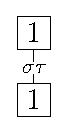
\includegraphics[width=.1\textwidth,height=.25\textheight]{MNG11symb}
  \includegraphics[width=.22\textwidth]{MNG11init}
  \includegraphics[width=.22\textwidth]{MNG11final}
  \end{figure}
\end{frame}

\begin{frame}%[allowframebreaks]
  \frametitle{Gluing (larger) solutions, time example}
  \begin{figure}
  \includegraphics[width=.9\textwidth]{MNG_ppo1ppo2_time}
  \end{figure}
\end{frame}

\begin{frame}%[allowframebreaks]
  \frametitle{Gluing (larger) solutions, space example}
  \begin{figure}
  \includegraphics[width=.6\textwidth]{MNG_ppo1ppo2_space}
  \end{figure}
\end{frame}

\begin{frame}%[allowframebreaks]
  \frametitle{Gluing (larger) solutions, space example}
  \begin{figure}
  \includegraphics[width=.3\textwidth]{MNG_ppo4ppo3_space}
  \end{figure}
\end{frame}


\begin{frame}
\frametitle{New solutions from gluing together old}
    \begin{figure}
    \begin{minipage}[height=.3\textheight]{.5\textwidth}
    \includegraphics[width=.7\textwidth,height=.3\textheight]{MNG_approxsymbdyn}
    \end{minipage}
    \end{figure}
\end{frame}

\begin{frame}
\frametitle{New solutions from gluing together old}
\begin{figure}
\begin{minipage}[height=.48\textheight]{.48\textwidth}
\centering \small{\texttt{(a)}}\\
\includegraphics[width=.8\textwidth,height=.4\textheight]{MNG_ppo_without_HOD}
\end{minipage}
\begin{minipage}[height=.48\textheight]{.48\textwidth}
\centering \small{\texttt{(b)}}\\
\includegraphics[width=.8\textwidth,height=.4\textheight]{MNG_ppo_subdomain_HOD}
\end{minipage}
\end{figure}
\end{frame}

\begin{frame}
\frametitle{New solutions from gluing together old}
\begin{figure}
\begin{minipage}[height=.20\textheight]{.5\textwidth}
\centering \small{\texttt{(a)}}
\includegraphics[width=.7\textwidth,height=.15\textheight]{MNG_ppo_subdomain2}
\end{minipage}
\begin{minipage}[height=.20\textheight]{.5\textwidth}
\centering \small{\texttt{(b)}}
\includegraphics[width=.7\textwidth,height=.15\textheight]{MNG_ppo_subdomain1}
\end{minipage}
\begin{minipage}[height=.20\textheight]{.5\textwidth}
\centering \small{\texttt{(c)}}
\includegraphics[width=.7\textwidth,height=.15\textheight]{MNG_ppo_subdomain0}
\end{minipage}
\end{figure}
\end{frame}

\begin{frame}
\frametitle{New solutions from gluing together old}
\begin{figure}
\begin{minipage}[height=.2\textheight]{.5\textwidth}
\centering \small{\texttt{(a)}}\\
\includegraphics[width=.5\textwidth,height=.2\textheight]{MNG_ppo_tiling_init_0}
\end{minipage}
\begin{minipage}[height=.2\textheight]{.5\textwidth}
\centering \small{\texttt{(b)}}\\
\includegraphics[width=.5\textwidth,height=.2\textheight]{MNG_ppo_tiling_final_0}
\end{minipage}
\begin{minipage}[height=.2\textheight]{.5\textwidth}
\centering \small{\texttt{(c)}}\\
\includegraphics[width=.5\textwidth,height=.2\textheight]{MNG_ppo_L30_T44}
\end{minipage}
\end{figure}
\end{frame}

\begin{frame}
\frametitle{New solutions from gluing together old}
\begin{figure}
\begin{minipage}[height=.48\textheight]{.48\textwidth}
\centering \small{\texttt{(a)}}\\
\includegraphics[width=.8\textwidth,height=.4\textheight]{MNG_ppo_without_HalfD}
\end{minipage}
\begin{minipage}[height=.48\textheight]{.48\textwidth}
\centering \small{\texttt{(b)}}\\
\includegraphics[width=.8\textwidth,height=.4\textheight]{MNG_ppo_subdomain_HalfD}
\end{minipage}
\end{figure}
\end{frame}

\begin{frame}
\frametitle{New solutions from gluing together old}
\begin{figure}
\begin{minipage}[height=.20\textheight]{.5\textwidth}
\centering \small{\texttt{(a)}}
\includegraphics[width=.7\textwidth,height=.15\textheight]{MNG_ppo_subdomain2_1}
\end{minipage}
\begin{minipage}[height=.20\textheight]{.5\textwidth}
\centering \small{\texttt{(b)}}
\includegraphics[width=.7\textwidth,height=.15\textheight]{MNG_ppo_subdomain1_1}
\end{minipage}
\begin{minipage}[height=.20\textheight]{.5\textwidth}
\centering \small{\texttt{(c)}}
\includegraphics[width=.7\textwidth,height=.15\textheight]{MNG_ppo_subdomain0_1}
\end{minipage}
\end{figure}
\end{frame}

\begin{frame}
\frametitle{New solutions from gluing together old}
\begin{figure}
\begin{minipage}[height=.30\textheight]{.6\textwidth}
\centering \small{\texttt{(a)}}\\
\includegraphics[width=.3\textwidth,height=.3\textheight]{MNG_ppo_tiling_init_pretruncation_1}
\end{minipage}
\begin{minipage}[height=.30\textheight]{.6\textwidth}
\centering \small{\texttt{(b)}}\\
\includegraphics[width=.3\textwidth,height=.3\textheight]{MNG_ppo_tiling_init_1}
\end{minipage}
\end{figure}
\end{frame}

\begin{frame}
\frametitle{New solutions from gluing together old}
\begin{figure}
\begin{minipage}[height=.30\textheight]{.6\textwidth}
\centering \small{\texttt{(a)}}\\
\includegraphics[width=.3\textwidth,height=.3\textheight]{MNG_ppo_tiling_final_1}
\end{minipage}
\begin{minipage}[height=.30\textheight]{.6\textwidth}
\centering \small{\texttt{(b)}}\\
\includegraphics[width=.3\textwidth,height=.3\textheight]{MNG_ppo_L30_T44}
\end{minipage}
\end{figure}
\end{frame}

\begin{frame}
\bea
u(\conf,\zeit) &=& \sum_{m,n} \cos(q_m \conf) (a_{mn}\cos(\omegan \zeit) + b_{mn}\sin(\omegan \zeit)) \continue
                &+& \sin(q_m \conf) (c_{mn}\cos(\omegan \zeit) + d_{mn}\sin(\omegan \zeit)).
\eea
\end{frame}


\begin{frame}
\bea
\Refl \tau u(\conf, \zeit) &=& \sum_{m,n} (-1)^{n+1} \cos(q_m \conf) (a_{mn}\cos(\omegan \zeit) + b_{mn}\sin(\omegan \zeit))\continue
                                &+& (-1)^{n} \sin(q_m \conf) (c_{mn}\cos(\omegan \zeit) + d_{mn}\sin(\omegan \zeit)) \, ,
\eea

Because \ppo\ s are invariant under this symmetry transformation, we can see by the prefactors of $(-1)^{n+1},(-1)^{n}$ that
this can only equate to the original expansion if the following conditions are met,

\bea
a_{mn},b_{mn} &=& 0 \, \mbox{for}\, n \, \mbox{even} \continue
c_{mn},d_{mn} &=& 0 \, \mbox{for}\, n \, \mbox{odd}
\eea

\end{frame}


\begin{frame}
  \frametitle{Application of ideas to quasi 2D Kolmogorov flow}
  Selection rules for spatiotemporal Fourier coefficients for \eqva\

  \bea
  a_{jk},b_{jk} &=& 0 \, \mbox{for}\, k \, \mbox{even multiple of forcing index} \ell \continue
  d_{jk},f_{jk} &=& 0 \, \mbox{for}\, k \, \mbox{odd multiple of forcing index} \ell
  \eea

  Total number of Fourier coefficients for shift-reflection invariant subspace.
  $N_x*\frac{N_y}{2*\ell}$

\end{frame}


\begin{frame}
\frametitle{Application of ideas to quasi 2D Kolmogorov flow}
\bea
d_{jkn},f_{jkn},m_{jkn},p_{jkn} &=& 0 \, \mbox{for}\, n \, \mbox{odd} \continue
a_{jkn},b_{jkn},g_{jkn},h_{jkn} &=& 0 \, \mbox{for}\, n \, \mbox{even}
\eea

For $k_y$ being an even number of multiples of the forcing profile index $\ell$, we have the following constraints

\bea
d_{jkn},f_{jkn},m_{jkn},p_{jkn} &=& 0 \, \mbox{for}\, n \, \mbox{even} \continue
a_{jkn},b_{jkn},g_{jkn},h_{jkn} &=& 0 \, \mbox{for}\, n \, \mbox{odd}
\eea

The number of Fourier coefficients is $N_x*\frac{N_y}{\ell}*\frac{N_t}{2}$
\end{frame}


\begin{frame}
\frametitle{Application of ideas to quasi 2D Kolmogorov flow}
Possible schematic for how to find periodic orbits in Kolmogorov flow in experiment
\begin{itemize}
\item Find periodic orbits with doubly periodic boundary conditions.
\item Use these periodic orbits (entire time discretization) as a seed for
initial condition using experimental boundary conditions.
\end{itemize}
\end{frame}


\begin{frame}
\bea
0&=& -\ii \omegan \Omega_{kx,ky,n}+ \frac{|\mathbf{k}|^2}{Re}\Omega_{kx,ky,n} \continue
 &+& \mathcal{F}(\nabla\times(\nabla^{-2}\mathcal{F}^{-1}(\Omega))\star\mathcal{F}^{-1}(\Omega)) \continue
 &+&\frac{\ell}{2}\mathcal{F}_t (\delta_{k_x}\delta_{|k_y|-\ell})
\eea
\end{frame}

%\begin{frame}[allowframebreaks]
%  \frametitle{References}
%  \scriptsize{\bibliographystyle{apalike}}
%  \bibliography{../../bibtex/siminos}
%\end{frame}




\end{document}
